\chapter{急性肾衰竭}

\section{前沿学术综述}

急性肾衰竭(acute renal
failure,ARF)是严重威胁重症患者生命的常见疾病。流行病学调查显示,重症医学科中急性肾衰竭的患病率高达31%~78%。对需要肾脏替代治疗的重症患者的研究也显示,在疾病严重程度类似的情况下,伴有急性肾衰竭患者的死亡风险增高4倍。急性肾衰竭成为影响和决定重症患者预后的关键性因素之一。加强重症医学科中急性肾衰竭的早期诊断、积极防治、逆转急性肾衰竭的发生发展,对改善重症患者的预后至关重要。

\subsubsection{急性肾衰竭的早期诊断与分级标准}

早期诊断是防治急性肾衰竭的关键。目前,急性肾衰竭已受到临床广泛的重视,诊断标准多达30多个,治疗措施也取得长足进步,但尚缺乏统一的诊断标准,尤其缺乏早期诊断标准。例如以需要肾脏替代治疗作为诊断标准,这类患者的肾衰竭实际上已达到终末阶段,使早期治疗无从谈起,造成治疗延误。

诊断标准不统一不但造成诊断和治疗的延误,且造成流行病学研究结果不具可比性。文献报道,重症医学科中急性肾衰竭的患病率为1%~31%,而病死率也从19%到83%不等。诊断标准中肾功能损害程度与病死率明显相关,若以轻度肾功能损害为标准,则病死率明显降低,而以严重肾功能损害为标准,则病死率明显增加。

因此,急性肾衰竭理想的诊断标准应既能实现急性肾衰竭早期诊断,又能准确反映其严重程度,并在临床能够易于理解和施行。同时,对急性肾衰竭应进行不同阶段的动态观察与诊治。早期诊断有助于早期防治,是降低急性肾衰竭重症患者病死率的关键,但对急性肾衰竭终末阶段的研究和观察同样是重要的,如肾脏替代性治疗的疗效评估、终末期肾衰竭对其他器官的影响与治疗,这也是目前存在众多不同诊断标准的原因之一。

目前诸多的诊断标准具有以下特点:①常用溶质清除能力间接反映肾功能,如血肌酐浓度;②用单位时间的尿量反映肾功能的急剧恶化,通常以24小时尿量<400~500ml,或每小时尿量<0.5ml/kg持续24小时为诊断标准;③对既往有肾脏损害病史者,采取不同标准。这些特点对于建立新的诊断标准仍具有借鉴意义。

鉴于急性肾衰竭诊断标准中存在的诸多问题,由危重病和肾脏病专家组成的急性透析质量控制倡议组织(acute
dialysis quality initiative
group,ADQI)在2004年第二次国际共识会议中,提出了急性肾衰竭的共识性分层诊断标准(表\ref{tab11-1})
\protect\hyperlink{text00017.htmlux5cux23ch1-16}{\textsuperscript{{[}1{]}}}
,该标准试图涵盖从存在急性肾损伤危险性开始,到急性肾损伤的最严重阶段------肾衰竭的全过程,包括急性肾损伤危险(risk,R)、急性肾损伤(injury,I)、急性肾衰竭(failure,F)三个阶段,同时这一标准也包括了肾功能丧失(loss,L)和终末期肾功能丧失(end-stage
kidney
disease,E)两个终末肾损害阶段,将这5个层次的英文第一个字母连在一起,即RIFLE,因此,该急性肾损伤的分层诊断标准也称为RIFLE分层标准。

\begin{table}[htbp]
\centering
\caption{急性肾功能损伤的RIFLE分层诊断标准}
\label{tab11-1}
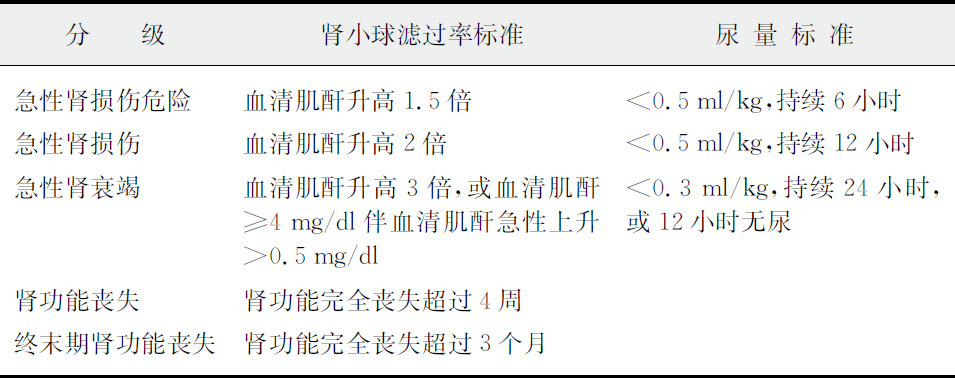
\includegraphics{./images/Image00085.jpg}
\end{table}

RIFLE分层诊断标准首先解决了急性肾衰竭的早期诊断问题,使临床早期诊断成为可能。该标准同时也包含了急性肾损害最严重的阶段------急性肾衰竭的诊断,并对终末期的肾功能丧失进行了定义。

当然,RIFLE分层诊断标准的价值,还取决于其对急性肾损害的分层是否能够准确反映重症患者的预后。研究发现若以RIFLE标准对重症患者进行预后评估,67%的重症患者发生急性肾损害,其中急性肾损伤危险、急性肾损伤和急性肾衰竭分别占12%、27%和28%。未合并急性肾功能损害的患者病死率仅5.5%,而发生急性肾功能损害者病死率明显增加,根据RIFLE标准对肾损害程度进行分层,急性肾损伤危险、急性肾损伤和急性肾衰竭的病死率依次显著增加,分别为8.8%、11.4%和26.3%。可见,RIFLE分层标准能够有效反映重症患者的预后,且有助于急性肾损害的早期诊断,值得在重症患者中推广应用。

自RIFLE诊断标准发表至今,全球已有超过55万人使用了该标准,引用该标准的原始文献超过17万篇,已达到对急性肾损伤诊断标准化的目的。

随着RIFLE标准的广泛使用,其缺陷也逐渐暴露出来,引起人们的关注:RIFLE标准忽视了肌酐和尿量的轻微改变,然而近年来越来越多的研究认为肌酐值升高150%过于保守,轻微肌酐值变化对预后也有极大的影响。基于这些原因,2005年9月急性肾损伤网络(acute
kidney injury
network,AKIN)专家组在阿姆斯特丹召开会议对RIFLE标准进行了讨论和修正,并于2007年发布了新的标准(AKIN标准)。根据该标准,将急性肾损伤定义为:不超过3个月的肾脏功能或结构方面的异常,包括血、尿、组织检测或影像学方面的肾损伤标志物的异常,其诊断要点为:肾功能突然减退,患者在48小时内血清肌酐升高绝对值≥26.4μmol/L(0.3mg/dl);或血清肌酐值较基线升高≥50%;或每小时尿量<0.5ml/kg、时间超过6小时。具体分级标准见表\ref{tab11-2}。

\begin{table}[htbp]
\centering
\caption{急性肾功能损伤的AKIN分层诊断标准}
\label{tab11-2}
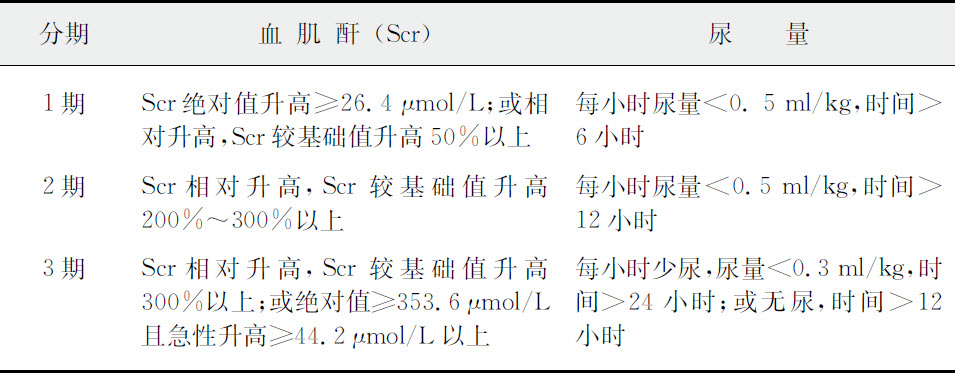
\includegraphics{./images/Image00086.jpg}
\end{table}

与RIFLE诊断标准相比较,AKIN诊断标准做了5个方面的修改:①保留了RIFLE诊断标准的3个急性期变化,但取消了R、I和F分期名称,改为数字分期,1、2、3期基本对应于RIFLE的R、I和F分期;②取消了肾小球率过滤变化标准,单纯采用肌酐标准;③在1期诊断标准中增加了血清肌酐绝对值升高≥26.4μmol/L(0.3mg/dl),肌酐变化值更小,可能提高了诊断的敏感性;④将所有接受肾脏替代治疗的患者划分为急性肾损伤3期,相当于RIFLE标准的衰竭期(failure);⑤取消了RIFLE诊断标准中判断预后分级的两个分期(L期和E期)。

AKIN标准将诊断时限限制在48小时以内,强调了血肌酐的动态变化,这样改动是考虑可能会带来以下好处:①排除了肾功长期缓慢改变带来的误诊;②采用肌酐绝对值变化作为诊断标准,肌酐变化值更小,同时避免了基础值无法确定所带来的诊断困难,为临床上急性肾损伤的早期诊断和干预提供了可能性;③对于造成肌酐和尿量短期急剧改变的可早期纠正的“可逆性”病因,如容量不足或尿路梗阻,提供了充足的复苏和纠正时间,有助于提供更准确的诊断。

基于现有的关于RIFLE和AKIN诊断标准的比较研究,还无法得出AKIN标准优于RIFLE标准的结论
\protect\hyperlink{text00017.htmlux5cux23ch2-16}{\textsuperscript{{[}2{]}}}
,仍需大规模的前瞻性研究评估不同分层标准对急性肾衰竭的早期诊断价值及预后价值。

\subsubsection{重症医学科中急性肾衰竭的早期防治}

鉴于急性肾衰竭是导致重症患者预后凶险的重要原因,重症医学科的重症患者是急性肾衰竭的高危人群,早期预防急性肾衰竭显得十分重要。针对重症医学科中导致急性肾衰竭的常见原因,采取目标导向性的预防策略,有可能降低急性肾衰竭的患病率。

(1)严重感染导致的急性肾衰竭 严重感染和感染性休克是导致急性肾衰竭的常见原因。严重感染者中有9%~40%的患者最终发生急性肾衰竭,感染的严重程度明显影响急性肾衰竭发生率,反之,发生急性肾衰竭也进一步增加严重感染患者的病死率。Bagshaw等对33375名全身感染患者调查发现,42.1%的患者并发急性肾损伤;全身感染所致的急性肾损伤往往病情更重,住重症医学科时间更长,死亡率更高
\protect\hyperlink{text00017.htmlux5cux23ch3-16}{\textsuperscript{{[}3{]}}}
。严重感染的患者并发急性肾衰竭的病死率高达70%,明显高于其他原因所致急性肾衰竭的病死率。可见早期防治严重感染导致的急性肾衰竭,对于最终改善严重感染的预后具有重要临床价值。

缺血和炎症性损伤是严重感染导致急性肾衰竭的主要机制。内毒素诱发的复杂炎症和免疫网络反应等多个方面,参与了感染性急性肾损伤的发病,并可能成为其主要机制。有研究证实,感染性急性肾损伤的肾脏局部会释放TNF-α等炎症因子,并引起肾小管细胞凋亡
\protect\hyperlink{text00017.htmlux5cux23ch4-16}{\textsuperscript{{[}4{]}}}
。上世纪90年代以来,针对控制炎症反应的炎性细胞因子单克隆抗体或阻断剂的研究一度给严重感染的治疗和急性肾衰竭的预防带来希望,然而,不仅单克隆抗体价格昂贵,且所有的临床研究均以失败告终,看来试图单纯阻断少数炎性介质来控制复杂的炎症反应网络,进而控制严重感染、预防急性肾衰竭的目标目前仍难以实现。积极纠正严重感染的低血容量状态,逆转肾脏缺血,成为急性肾衰竭防治的希望。

严重感染时肾脏低灌注是导致急性肾衰竭的重要原因,早期强化的目标性血流动力学管理是纠正肾脏低灌注的有效途径。Rivers等学者在严重感染或感染性休克发生6小时内,通过积极液体复苏使中心静脉压达到8~12mmHg(1mmHg=0.133kPa),以纠正有效循环血容量不足,若平均动脉压仍低于65mmHg,则加用血管活性药物,恢复有效组织灌注。监测每小时尿量,使每小时尿量>0.5ml/kg。同时监测中心静脉血氧饱和度或混合静脉血氧饱和度,若中心静脉血氧饱和度<70%,补充红细胞悬液,使血细胞比容>30%,以此重建和维持氧需与氧供的平衡。若6小时内实现早期目标导向治疗,严重感染的病死率可从46.5%降至30.5%,且急性肾衰竭的发生率也明显降低
\protect\hyperlink{text00017.htmlux5cux23ch5-16}{\textsuperscript{{[}5{]}}}
。早期有效的改善肾脏灌注成为预防严重感染患者发生急性肾衰竭的有效途径。至于早期液体复苏中液体种类对急性肾衰竭发生的影响,目前尚无确切的证据说明胶体溶液和晶体溶液孰优孰劣,但是就恢复有效循环血量的速度和效率而言,胶体溶液明显优于晶体溶液。

近年来,不同血管活性药物在急性肾衰竭防治中的地位备受关注。以往认为,多巴胺具有选择性肾血管扩张和增加尿量的作用,肾脏剂量(小剂量)的多巴胺长期在临床上被广泛用于急性肾衰竭的防治。但大量的研究表明,每分钟3~5μg/kg多巴胺对肾脏血管并无血管扩张作用,甚至有轻度的缩血管作用;小剂量多巴胺增加尿量与其轻度抑制近曲小管钠的重吸收有关,并不增加肌酐清除率;小剂量多巴胺既不能预防重症患者发生急性肾衰竭,对病死率也无影响;另外,多巴胺也存在明显不良作用,除引起心动过速外,还对垂体前叶激素具有抑制作用,抑制T细胞功能,抑制呼吸中枢兴奋性,并可减少肠道灌注。总的来讲,小剂量多巴胺并无肾脏保护作用,临床上不应常规应用。

去甲肾上腺素越来越多地应用于感染性休克的治疗,其有可能对急性肾衰竭具有预防作用。在正常人和动物中,去甲肾上腺素明显减少肾血流量和尿量,但在严重感染的情况下,去甲肾上腺素能够明显改善感染性休克患者的肾小球滤过率,并增加尿量。前瞻性研究显示,去甲肾上腺素组的病死率明显低于多巴胺组,但目前尚缺乏去甲肾上腺素对感染性休克急性肾衰竭预防效应的直接依据。

血管加压素一般用于大剂量常规升压药无效的顽固性感染性休克。最近的研究显示,血管加压素对肾脏可能具有保护作用。肾小球滤过率主要由入球小动脉和出球小动脉的压力差决定,血管加压素收缩出球小动脉更明显,使肾小球滤过压明显增加,进而增加肾小球滤过率和尿量,发挥肾保护作用。已有小样本临床研究显示,血管加压素能够预防感染性休克患者发生急性肾衰竭,并明显优于其他血管活性药物,但仍需要多中心的随机对照研究进一步证实。

(2)药物导致的急性肾衰竭 具有肾毒性药物易于引起或加重肾功能损害,如氨基糖苷类、万古霉素和两性霉素B等常用药物。避免应用肾毒性药物或采用更为合理的用药方法,有可能预防急性肾衰竭的发生。

重症患者应用氨基糖苷类药物导致肾功能损害的发生率高达10%。氨基糖苷类药物主要通过肾小球滤过,在肾小管中部分被重吸收,并积聚在小管上皮细胞溶酶体中,其肾损害主要与溶酶体破坏和肾小管上皮细胞膜损伤导致小管细胞坏死有关。氨基糖苷类药物是否导致肾损害,不仅与肾小管中药物浓度与作用时间有关,还与治疗疗程、既往是否具有肾损害病史有关。

(3)造影剂导致的急性肾衰竭 影像学诊断应用的造影剂或增强剂可诱导急性肾衰竭,占医院获得性急性肾衰竭的10%。尽管肾功能正常者应用造影剂后急性肾损害的发生率很低,但已有轻度肾损害者应用造影剂后急性肾损害的发生率可达5%,而已有明显肾功能损害或糖尿病者,应用造影剂后急性肾损害的发生率可高达50%。可见,基础肾功能状态也是决定造影后是否发生急性肾损害的重要因素。

总之,重症患者一旦发生急性肾衰竭,预后凶险,应用RIFLE及AKIN标准有助于实现急性肾损伤的早期诊断和治疗,并利于对高危患者采取积极措施,预防急性肾衰竭的发生,有可能最终改善重症患者的预后。

\section{临床问题}

\subsection{急性肾衰竭的病因与临床特征}

\subsubsection{重症患者发生急性肾衰竭的危险因素有哪些?}

一般认为,低血压/休克、充血性心衰、全身性感染、糖尿病、氨基糖苷类抗生素应用、造影剂应用、高胆红素血症、机械通气、外科大手术、肾移植等因素是发生急性肾衰竭的独立危险因素。

(1)全身性感染 全身性感染是急性肾衰竭患病最重要的独立危险因素。Brivet的研究显示急性肾衰竭的主要患病因素中,48%为全身性感染。不但院内感染与急性肾衰竭的发病有关,社区获得性感染也与急性肾衰竭患病密切相关。Rayner报道了239例社区获得性全身性感染患者,其中有24%的患者血清肌酐浓度升高1倍以上。

(2)肾毒性药物的应用 肾毒性药物的应用也是重要的独立危险因素。肾毒性药物引起的急性肾衰竭约占各种病因的35%。肾毒性药物很多,不同的肾毒性药物具有不同的肾损伤机制------①高张力性损害:葡聚糖、甘露醇等可导致肾脏发生高张性损伤;②缺血性损害:利尿剂、血管紧张素转换酶抑制剂、降压药等导致血容量不足和血压降低,使肾脏灌注减少而导致肾脏损害;③肾小管毒性损害:氨基糖苷类药物、万古霉素、两性霉素B、放射造影剂、重金属等对肾小管具有直接损害作用,Ⅳ型免疫球蛋白、葡聚糖、麦芽糖、蔗糖、甘露醇等可导致肾小管肿胀;④肾血管内皮细胞损害:环胞素A、丝裂霉素C、可卡因、雌激素、奎宁等药物可导致肾脏毛细血管内皮细胞损伤;⑤入/出球小动脉舒缩异常:非甾体抗炎药、放射造影剂、两性霉素B等可导致入球小动脉痉挛,降低肾小球滤过率。血管紧张素转换酶抑制剂、血管紧张素Ⅱ受体拮抗剂等药物可导致出球小动脉扩张,降低肾小球滤过率;⑥结晶尿:磺胺药物、无环鸟苷、蛋白酶抑制剂等药物可在肾小管内结晶,导致肾小管功能损害;⑦肾小球损害:金制剂、青霉胺、非甾体抗炎药等可直接损伤肾小球;⑧间质性肾炎:多种药物可导致间质性肾炎;⑨色素性肾小管功能损害:肌红蛋白尿和血红蛋白尿可导致肾小管损害。

(3)重大手术 重大手术也是急性肾衰竭患病的高危因素之一。Liano报道的748例急性肾衰竭患者中,有27%为术后患者。研究显示心脏术后患者急性肾衰竭患病率为0.4%~7.5%,而非心脏大手术患者的急性肾衰竭患病率为0.6%。心脏术后的肾功能障碍是影响患者生存的独立因素,其比值是无肾功能障碍的7.9倍,因此重大手术患者应特别注意急性肾衰竭的早期预防和治疗。

重大手术后患者易发生急性肾衰竭的原因,主要与下列因素有关:①患者具有糖尿病、高血压、血管性疾病、充血性心衰等慢性疾病,导致患者肾脏功能贮备降低,基础肾小球滤过率下降;②麻醉和手术应激导致肾小球入球小动脉收缩,肾小球滤过率降低;③术后并发全身性感染、休克、心衰等并发症,或应用肾毒性药物,或二次手术,构成对肾脏的二次打击,极易导致急性肾衰竭。

\subsubsection{急性肾衰竭的主要病因分型有哪几类?}

急性肾衰竭的病因复杂,根据致病因素在肾脏直接作用的部位,可分为肾前性因素、肾性因素和肾后性因素。

(1)肾前性急性肾衰竭 主要与血容量不足和心脏泵功能明显降低导致肾脏灌注不足有关,在急性肾衰竭中最为常见,占30%~60%。反映了当前重症患者治疗中,对容量状态或肾脏灌注缺乏足够的重视,或对容量估计严重不足。肾前性肾衰是医院获得性肾衰的主要原因之一。

各种肾前性因素引起血管内有效循环血量减少,肾脏灌注量减少,肾小球滤过率降低,并使肾小管内压力低于正常;流经肾小管的原尿减少,速度减慢,因此尿素氮、水及钠的重吸收相对增加,从而引起血尿素氮升高,尿量减少及尿比重增高的现象,称为肾前性氮质血症。因肾小管对钠的重吸收相对增加,使尿钠排出减少,钠排泄比例明显降低、肾衰竭指数降低(<1mmol/L),因尿少、尿素氮重吸收相对增加,出现尿素氮和血肌酐浓度不成比例的增高(即球管间不平衡现象),血尿素氮可高达37.5mmol/L(100mg/dl)以上,而血肌酐则仅稍高于正常,尿与血的肌酐比例明显升高。

引起肾前性急性肾衰竭的原因常常包括:①低血容量,由于严重外伤、烧伤、挤压综合征、大出血、外科手术、脱水、胰腺炎、呕吐、腹泻或大量应用利尿剂所致;②有效血容量减少,由于肾病综合征、肝衰竭、全身性感染、休克、应用血管扩张剂或麻醉药所致;③心输出量减少,由于心源性休克、心肌梗死、严重心律紊乱、充血性心功能衰竭、心包填塞及急性肺梗死所致;④肾血管阻塞,由于肾静脉或肾动脉栓塞,或动脉粥样变所致;⑤肾血管的自身调节紊乱,由于前列腺素抑制剂、血管紧张素转化酶抑制剂、环孢菌素A的作用所致。

(2)肾性急性肾衰竭 肾性急性肾衰竭是肾实质疾患所致,或由于肾前性病因未能及时解除而发生肾实质病变,占急性肾衰竭的20%~40%。在考虑急性肾衰竭的肾性因素时,应考虑到肾脏的各个解剖结构是否发生病变,不但应考虑到肾血管、肾小球的病变,还应注意肾间质和肾小管等解剖结构的病变。当然,需要注意的是,尽管急性肾脏血管病变(如动脉栓塞、血管炎、血栓形成等)、肾小球病变(如肾小球肾炎等)、间质性病变(如过敏性间质性肾炎等)均是急性肾衰竭的病因之一,但急性肾衰竭、特别是医院获得性急性肾衰竭最重要的病因仍然是急性肾小管损伤。急性肾小管坏死往往与肾脏缺血和肾毒性药物的应用有关。

归纳起来,急性肾性肾衰的病因主要包括:①肾小管疾患,为急性肾衰竭的主要病因,其中以急性肾小管坏死最为常见,肾缺血、肾中毒(药物、造影剂、重金属、有机溶剂、蛇毒、中草药)及高钙血症等均可引起肾小管损伤,导致急性肾衰竭;②肾小球疾患,多数患者表现为少尿型肾衰,占87.5%,非少尿型占14.3%;③急性肾间质性疾患,主要因严重感染、全身性感染及药物过敏或由于淋巴瘤、白血病或肉瘤病变侵及肾间质所致;④肾脏血管疾病,肾脏的小血管炎或大血管疾患;⑤慢性肾脏疾病急性恶化,某些诱因致使病情急剧恶化,肾功能急骤减退也可导致急性肾衰竭。

(3)肾后性急性肾衰竭 各种原因引起的急性尿路梗阻(如腔内阻塞或外部压迫等),导致急性肾衰竭,归结为肾后性急性肾衰竭,临床上较为少见,占急性肾衰竭的1%~10%。如诊断和治疗及时,这类肾衰竭往往可恢复。

肾以下尿路梗阻使梗阻上方的压力增高,甚至发生肾盂积水,肾实质受压使肾功能急剧下降。肾后性急性肾衰竭可见于:①结石、肿瘤、血块、坏死肾组织或前列腺增生所致的尿路梗阻;②肿瘤蔓延、转移或腹膜后纤维化所致的粘连、压迫输尿管而引起梗阻。

\subsubsection{急性肾衰竭少尿期有哪些临床特征?}

急性肾小管坏死病因不一,起始表现也不同,一般起病较急骤,全身症状明显。根据临床表现和病程的共同规律,一般分为少尿期、多尿期和恢复期3期。少尿期的临床特征主要包括:

(1)尿量减少 尿量骤减或逐渐减少,每日尿量持续少于400ml者为少尿,少于100ml者为无尿。急性肾小球坏死患者罕见完全无尿,持续无尿者预后极差。由于致病原因不同,病情轻重不一,少尿持续时间不一致,一般为1~2周,但可短至数小时或长达3个月以上。一般认为肾中毒者持续时间短,而缺血性者持续时间较长。若少尿持续4周以上应重新考虑急性肾小管坏死的诊断,有可能存在肾皮质坏死、原有肾疾患或肾乳头坏死等。

非少尿型急性肾小管坏死,指患者在氮质血症期每日尿量持续在500ml以上,甚至1000~2000ml。非少尿型的发病率近年有增加趋势,高达30%~60%。

(2)进行性氮质血症 由于肾小球滤过率降低引起少尿或无尿,致使排出氮质和其他代谢物质减少,血浆肌酐和尿素氮升高,其升高速度与体内蛋白分解状态有关。在无并发症且治疗恰当的病例,每日血尿素氮上升速度较慢,为3.6~7.1mmol/L(10~20mg/dl),血浆肌酐浓度上升仅为44.2~88.4μmol/L(0.5~1.0mg/dl)。但在高分解状态时,如伴广泛组织创伤、全身性感染等,每日尿素氮可升高10.1~17.9mmol/L(30~50mg/dl),肌酐每日升高176.8μmol/L(2mg/dl)或以上。促进蛋白分解的因素尚有热量供给不足、肌肉坏死、血肿、胃肠道出血、感染、发热、应用糖皮质激素等。

(3)水、电解质紊乱和酸碱平衡紊乱 包括水中毒、高钾血症、代谢性酸中毒、低钙血症、高磷血症、低钠血症和低氯血症等。

水过多:见于水分控制不严,摄入量或补液量过多,失水量如呕吐、出汗、伤口渗液量等估计不准确以及液体补充时忽略计算内生水。随少尿期延长,易发生水过多,表现为稀释性低钠血症,软组织水肿、体重增加、高血压、急性心功能衰竭和脑水肿等。

高钾血症:①由于尿液排钾减少,如同时体内存在高分解状态,导致细胞内钾离子释放入血;②挤压时肌肉坏死、血肿和感染等或酸中毒时细胞内钾转移至细胞外,有时可在几小时内发生严重高钾血症;③静脉内滴注大剂量的青霉素钾盐(每100万单位青霉素钾盐1.6mmol);④大量库存血(库存10天血液每升含钾可达22mmol);⑤摄入含钾较多食物或饮料,均可引起或加重高钾血症。无并发症者每日血钾上升不到0.5mmol/L。高钾血症有时隐匿,可无特征性临床表现,或仅出现恶心、呕吐、手麻、心率减慢,直到后期出现室内、房室传导阻滞或心脏停搏。高钾对心肌毒性作用尚受体内钠、钙浓度和酸碱平衡的影响,当同时存在低钠、低钙血症或酸中毒时,高钾血症临床表现较显著,且易诱发各种心律失常。值得一提的是,血清钾浓度与心电图之间可存在不一致现象。高钾血症是常见的死因之一,早期透析可预防其发生。

代谢性酸中毒:正常人每日固定酸性代谢产物为50~100mmol。急性肾衰竭时,由于酸性代谢产物排出减少,肾小管泌酸能力和保存\ce{HCO3-}
能力下降等原因,致使每日血浆\ce{HCO3-}
浓度下降1~2mmol/L;在高分解状态时降低更多、更快。内源性固定酸大部分来自蛋白分解,少部分来自糖和脂肪氧化。\ce{HCO3-}
和其他有机阴离子均释放和堆积在体液中,导致本病患者阴离子间隙增高。酸中毒可降低心室颤动阈值。高钾血症、严重酸中毒和低钙低钠是急性肾衰竭的严重状况,在已接受透析治疗的病例较少见,但对严重肌肉组织坏死病例,特别是深部肌肉坏死者仍应警惕。

低钙血症、高磷血症:少尿2天后即可发生低钙血症。由于常同时伴有酸中毒,使细胞外液离子钙增多,故多不发生低钙常见的临床表现。高磷血症较常见,但罕见明显升高。

低钠血症和低氯血症:两者多同时存在,低钠血症主要是由于水过多所致稀释性低钠血症。严重低钠血症时,血浆渗透浓度降低,导致水分向细胞内渗透,出现细胞水肿,表现为急性水中毒和脑水肿症状,并进一步加重酸中毒。低氯血症除稀释性外,尚可因呕吐、腹泻等加重,可出现腹胀或呼吸表浅、抽搐等代谢性碱中毒表现。

(4)心血管系统表现 主要包括高血压、心功能衰竭等。

高血压:除肾缺血、肾素分泌增多因素外,水过多引起容量负荷过多可加重高血压。急性肾小管坏死早期高血压不多见,但若持续少尿,约1/3患者发生轻、中度高血压,血压一般在140~180/90~100mmHg,有时可更高,甚至出现高血压脑病,伴有妊娠者尤易发生。

心功能衰竭:主要为液体潴留引起,但高血压、严重心律失常和酸中毒等为影响因素。早年发生率较高,在采取严格控制水分和早期透析等措施后发生率已明显下降。

心律失常:除高钾血症引起窦性停搏、窦房传导阻滞、不同程度房室传导阻滞和束支传导阻滞、室性心动过速、心室颤动外,尚可因病毒感染和洋地黄应用等而引起室性早搏等心律失常的发生。

心包炎:早年发生率为18%,采取早期透析后降至1%。多表现为心包摩擦音和胸痛,罕见大量心包积液。

\subsubsection{急性肾衰竭多尿期和恢复期有何特点?}

进行性尿量增多是肾功能恢复的一个标志,每日尿量可成倍增加。一般认为,24小时尿量增加到400ml以上,提示急性肾衰竭进入多尿期。进入多尿期后,肾功能并不立即恢复,存在高分解代谢的患者血浆肌酐和尿素氮仍上升,当肾小球滤过率明显增加时,血氮质逐渐下降。多尿期早期仍可发生高钾血症,多尿期后期易发生低钾血症。另外,此期仍易发生感染、心血管并发症和上消化道出血等并发症。多尿期持续时间多为1~3周或更长。

恢复期患者自我症状缓解,血尿素氮和肌酐接近正常,尿量逐渐恢复正常。除少数外,肾小球滤过功能多在3~12个月内恢复正常,但部分病例肾小管浓缩功能不全可持续1年以上。若肾功能持久不恢复,提示肾脏遗留永久性损害。

\subsection{急性肾衰竭的临床诊断}

\subsubsection{急性肾衰竭的临床诊断思路是什么?}

急性肾衰竭的早期诊断对重症患者十分重要。要做到对急性肾衰竭迅速诊断,应首先排除肾前性和肾后性因素,然后确定肾脏本身的原因。一般可采用以下“四步法”进行急性肾衰竭的诊断。

第一步:了解既往病史和现病史,进行体格检查,导尿(特别是无尿患者),做尿液分析。

第二步:

(1)分析尿液检查结果(表\ref{tab11-3});

\begin{table}[htbp]
{\centering
\caption{肾前性氮质血症与急性肾衰竭(急性肾小管坏死)的尿液分析比较}
\label{tab11-3}
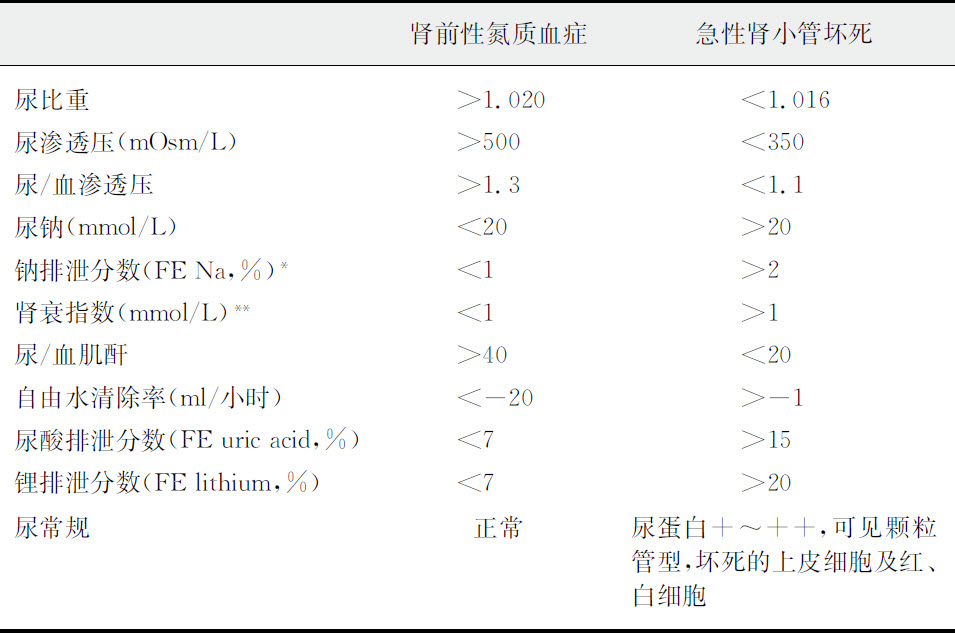
\includegraphics{./images/Image00090.jpg}}

\footnotesize
* 钠排泄分数=(尿钠×血肌酐)/(血钠×尿肌酐)×100%;

** 肾衰指数=尿钠×血肌酐/尿肌酐。
\end{table}



(2)评价尿路情况,排除尿路梗阻。可采用B超等检查手段;

(3)如需进一步了解患者血管内容量状态和心脏功能状态,可通过有创动脉压监测、中心静脉压监测、肺动脉漂浮导管监测及超声心动图(特别是食管超声)检查,对患者容量状态和心功能状态进行评价;

(4)如考虑肾小球肾病或血液系统恶性肿瘤,则应进一步进行血液学检查;

(5)如考虑肾脏血管病变,应通过同位素扫描、超声多普勒或血管造影,对肾血管情况进行评价。

第三步:根据急性肾衰竭病因,确定初步治疗方案。包括血容量补充、正性肌力药物的应用、解除尿路梗阻等措施。

第四步:为进一步明确诊断,可行肾脏活检,并根据初步诊断,采取经验性治疗。

一般情况下,通过“四步法”诊断步骤中的第一步,可初步明确急性肾衰竭的病因。通过了解现病史和既往史,可明确患者是否应用肾毒性药物、是否应用放射造影剂、是否有血容量不足、低血压等肾脏缺血因素、是否有大手术等肾脏损害的危险因素。

明确患者的容量状态,早期纠正低血容量状态或低心排状态,具有重要的价值。对于肾前性氮质血症患者,早期纠正肾脏的低灌注状态,可逆转氮质血症,防止急性肾衰竭发生。即使对于急性肾衰竭的患者,积极纠正低灌注状态,也有利于防止肾脏功能的进一步恶化,促进肾功能早期恢复。详细的体格检查,结合有关病史,往往可以得到患者容量状态的证据。

当患者容量状态判断较为困难时,放置肺动脉漂浮导管,监测心输出量、肺动脉嵌顿压和中心静脉压,可较准确地评价患者的容量状态和心脏功能状态,同时,可指导容量复苏/正性肌力药物等治疗措施的调整。在容量复苏或应用正性肌力药物时,应同时观察尿量和尿液分析的变化。

尿液分析是急性肾衰竭的重要诊断手段。肾前性和肾后性氮质血症患者的尿液检查往往是正常的。尿液镜检中发现大量的色素颗粒管型或上皮细胞管型,常提示肾缺血或肾毒性药物引起的急性肾衰竭。

显微镜下如发现血色素,而且与红细胞不成比例,提示患者的急性肾衰竭与横纹肌溶解或溶血引起的色素尿有关。

当患者有明显的蛋白尿、血尿,尿液检查中发现大量的红细胞管型,提示急性肾衰竭与急性肾小球肾炎或血管炎有关。

尿液出现大量白细胞管型,见于急性肾盂肾炎、间质性肾炎或肾小球肾炎。

尿液沉渣Hansel染色发现嗜酸性粒细胞,则为嗜酸性粒细胞尿,急性肾衰竭并非是肾小管损害的结果。

当患者无发热、皮疹、外周血嗜酸性粒细胞增加等全身性过敏反应表现时,应首先考虑嗜酸性粒细胞尿与药物引起的间质性肾炎有关。

对于动脉造影后出现急性肾衰竭的患者或存在周围血管病变的急性肾衰竭患者,如发现嗜酸性粒细胞尿,提示急性肾衰竭与动脉栓塞性肾血管病变有关。

尿比重、渗透压、尿钠浓度及钠排泄分数等尿液指标是诊断和评价急性肾衰竭的重要指标(表\ref{tab11-3})。肾前性氮质血症导致少尿的患者,往往具有正常的肾小管功能,而急性肾衰竭患者的肾小管功能明显受损,肾小管对溶质和水的重吸收功能明显减低,由此可通过尿液诊断指标对急性肾衰竭与肾前性氮质血症进行鉴别。

当然,尿液诊断指标并不是完全可靠的。尿液中电解质的结果受许多因素的影响。病情不同、治疗干预不同,尿液电解质就可能出现不同的结果。对于接受利尿剂治疗的患者,葡萄糖、尿酸、放射造影剂等可导致碳酸氢钠尿和渗透性利尿。而对于原发性肾上腺皮质功能不全的患者,容量不足引起肾前性氮质血症时,尽管患者存在血容量不足,尿钠排泄分数仍然明显升高。另外,由于慢性肾脏功能不全或间质性肾炎患者肾小管对钠的重吸收功能降低,当容量不足引起肾前性氮质血症时,尿钠的排泄仍然很多。还需注意的是,尿钠和尿钠排泄分数降低也并非肯定是肾前性氮质血症。全身性感染、放射造影剂、横纹肌溶解等原因导致的间质性肾损害,早期肾小管就具有正常功能。这应引起重症医学科医师的高度重视,以免延误诊断和治疗。在尿路梗阻、急性肾小球肾炎、急性间质性肾炎等情况下,尿液诊断指标的结果往往也是不可靠的。

\subsubsection{何谓肾小球滤过率?}

肾小球滤过率即在单位时间内(分钟)从双肾滤过的血浆的毫升数,为测定肾小球滤过功能的重要指标。实际上当某种存在于血中的溶质,如果能从肾小球滤过,肾小管内不被重吸收也不分泌,此时肾小球滤过率=尿液中溶质浓度×单位时间尿量/血浆溶质浓度。在这种情况下的肾小球滤过率就是每分钟有多少毫升血中的溶质被肾小球清除。

可见,用于评价肾小球滤过率的溶质应具备以下条件:①能够从肾小球滤过;②溶质不被肾小管吸收;③肾小管也不分泌或排泄该溶质。

\subsubsection{何为菊粉清除率?有何意义?}

菊粉是一种不带电荷的果糖聚合物,分子量5200道尔顿,无毒,不参与任何化学反应。可从静脉注入人体,不与血浆蛋白结合,主要分布于细胞外液。清除方式是只从肾小球滤过而不被肾小管重吸收或分泌,在体内既不能合成亦不能分解。可见,菊粉符合测定肾小球滤过率的要求,菊粉清除率可以准确反映肾小球滤过功能,是测定肾小球滤过率的“金标准”。

测定方法:患者于清晨空腹,静脉滴注10%的菊粉溶液,同时放置导尿管。到血浆中菊粉的浓度稳定在10mg/L水平,每分钟尿量稳定后,测尿中的菊粉浓度,代入公式:菊粉清除率=尿菊粉浓度×单位时间尿量/血浆菊粉浓度,就是患者的肾小球滤过率。菊粉清除率虽然精确,但测定时程序繁杂,不适于临床应用。

\subsubsection{为什么肌酐清除率可以评价肾功能?有何临床意义?}

肌酐清除率是评价肾脏功能最常用的方法,但在临床应用时,必须了解其生理代谢情况及其与肾脏功能的关系,才有可能对肾脏功能做出合理的评价。

(1)肌酐的代谢与生理 肌酐是人体内肌酸的代谢产物,肌酸量与肌肉量成正比。正常情况下,机体以比较稳定的速度产生肌酐,并释放入血液循环。再由血液循环带到肾脏,从尿中排出到体外。正常人肌酐的排泄主要通过肾小球的滤过作用,原尿中的肌酐不被肾小管重吸收,而且,正常情况下肾小管几乎不分泌肌酐。当然,正常情况下人体内的肌酐来源包括内生肌酐(体内肌酸分解而来)和外生肌酐(来自摄入的鱼、肉类食物),由于外源性肌酐不足以影响清晨空腹时的血肌酐测定,所以空腹时血肌酐水平是比较稳定的。正常人每日肌酐的产生量和排出量是相等的。

肌酐的分子量为113道尔顿,不被肾脏代谢,不与蛋白质结合,可以自由通过肾小球,不被肾小管重吸收,在血肌酐无异常增高时亦不为肾小管分泌,所以可用肌酐清除率代替菊粉清除率检测肾小球滤过率。

(2)肌酐清除率的测定方法 肌酐主要从肾小球滤过,但亦有时从肾小管排泌,故肌酐清除率并非十分理想的代表肾小球滤过率的指标,它高于肾小球滤过率的实际值,尤其在肾功能减退时。但检测方便,目前仍较广泛地应用来表示肾小球滤过率。

常规方法:以往的做法是素食3天后,收集24小时的全部尿液,在收集尿液结束时取血,测定血、尿中肌酐浓度,然后计算肌酐清除率。因收集24小时尿液较麻烦,全天血肌酐水平也有波动,在同一个人测多次肌酐清除率的结果,其误差可达25%,而且,少量外源性肌酐不影响次日清晨空腹血肌酐浓度。因此,目前多采取测清晨空腹血及取血前后共4小时全部尿量进行肌酐清除率测定,以减少误差,而且测量前不必素食。正常值为:80~120ml/分。

Cockcroft推算法:1976年Cockcroft和Gault提出以血肌酐值推算肌酐清除率的公式(性别不同,公式略有不同),但此公式对老年人、儿童及肥胖者不适用。

\[
\begin{array}{l}
    \text{男性肌酐清除率(ml/分)}=\frac{(140-\text{年龄}\times \text{体重(kg)}}{72\times \text{血肌酐(md/dl)}}\\
    \text{男性肌酐清除率(ml/分)}=\frac{(140-\text{年龄}\times \text{体重(kg)}}{85\times \text{血肌酐(md/dl)}}
\end{array}    
\]

1991年Giovannetti和Barsotti报道以菊粉清除率为标准评价肌酐清除率,包括肾功能正常及慢性肾衰竭者在内,其结果发现肌酐清除率的敏感性不比菊粉清除率差。而Desanto等亦以菊粉清除率为标准,将测定的肌酐清除率和用Cockcroft公式计算出的肌酐清除率进行比较,他们认为计算的肌酐清除率较实际测定的肌酐清除率更能真实反映肾小球滤过率。

西米替丁改良法:1996年Zaitzman等提出西米替丁改良法测定肌酐清除率,主要利用西米替丁竞争性强烈抑制肾小管对肌酐的分泌,使尿中肌酐完全来源于肾小球滤过,从而改善肌酐清除率作为肾小球滤过率标志的可靠性------口服西米替丁800mg,收集服药后45分钟内的尿液,同时在尿液收集结束时采血,测定尿液和血浆中肌酐浓度,计算肌酐清除率。

Zaitzman的研究显示西米替丁改良法测定的肌酐清除率与\textsuperscript{125}
I碘酞酸盐测定的肾小球滤过率(与菊粉清除率测定方法类似)比较,两者比值1.12±0.02。如不使用西米替丁,则比值为1.33±0.08。西米替丁改良法测定的肌酐清除率能够较准确的反映肾小球滤过率。

由于口服西米替丁的生物利用度为60%,口服后30分钟血浆浓度达到峰值,半衰期为2小时,因此,在口服西米替丁800mg后的3小时内均可较准确的测定肌酐清除率。

西米替丁改良法不但适用于肾脏功能轻度降低的重症患者,还特别适用于肾小球滤过率显著降低的急性肾衰竭患者。

\subsubsection{为什么要监测血肌酐?有何临床意义?}

血肌酐浓度是反映肾脏肾小球滤过率的常用指标之一。正常情况之下,体内肌酐产生的速度约为1mg/分。肌酐只从肾小球滤过并以同样速度清除。当肾小球滤过功能下降时,血肌酐即可上升。但研究证实,只有当肾小球滤过率下降到正常1/3时,血肌酐才明显上升,所以血肌酐测定并非敏感的测定肾小球过滤功能的指标。只有在肾功能不全失代偿时,血肌酐值才升高。

血肌酐的正常值应<1.5mg/dl(133μmol/L)。

性别、肌肉容积均在正常值范围内影响血肌酐的数值。当肌肉萎缩性病变的患者肌肉代谢减少时,血肌酐的浓度亦可稍低。

\subsubsection{血尿素氮异常能否说明患者肾功能异常?}

血尿素氮也是反映肾小球滤过率的常用指标之一。血中尿素氮是人体蛋白质代谢的终末产物。尿素的生成量取决于饮食中的蛋白质的摄入量,组织蛋白质的分解代谢及肝功能的情况。血液中的尿素全部从肾小球滤过,正常情况下约30%~40%被肾小管重吸收,肾小管亦可排泌少量的尿素,严重的肾衰竭时排泌量增加。血中的尿素氮的测定虽可以反映肾小球的滤过功能,但肾小球的滤过功能必须下降到正常的1/2以上时,尿素氮才会升高。故尿素氮的测定并非敏感的反映肾小球的滤过功能的指标。血尿素氮的正常值为8~21mg/dl(2.9~7.5mmol/L),其血液水平受多种因素的影响,如感染、高热、脱水、消化道出血、进食高蛋白饮食等均可影响血中尿素氮。血中尿素氮的上升不一定是肾小球的滤过功能受损的结果,临床上必须认真分析原因,鉴别真正导致血尿素氮上升的病因。

\subsubsection{血尿素氮/肌酐的临床意义如何?}

肾功能正常时,血尿素氮/肌酐通常为10。当血尿素氮>25mg/dl(8.9mmol/L)时即可诊断为氮质血症。当发生氮质血症且尿素氮/肌酐增高时,常说明此氮质血症是由于肾前因素引起(即由于各种原因引起的肾血流量的下降)。当氮质血症同时伴尿素氮/肌酐下降时,多为肾脏本身的实质性疾病引起所致,所以这一比值有助于鉴别氮质血症是由于肾前性因素还是肾性的因素引起。

\subsubsection{血β2 微球蛋白能够反映肾小球滤过功能吗?}

β\textsubscript{2}
微球蛋白是体内有核细胞,包括淋巴细胞、血小板、多形核白细胞产生的一种小分子球蛋白。其分子量为11800道尔顿,广泛存在于血浆、尿、脑脊液、唾液及初乳中,正常人血中的β\textsubscript{2}
微球蛋白浓度很低,平均约为1.5mg/dl。正常情况下可以自由通过肾小球,然后在近端肾小管内几乎全部被重吸收,当肾小球滤过功能下降时,血中的β\textsubscript{2}
微球蛋白水平上升,所以血β\textsubscript{2}
微球蛋白是反映肾小球滤过功能一个极好指标,与年龄无关,但当体内有炎症或肿瘤时,血中β\textsubscript{2}
微球蛋白增高,应注意鉴别。

\subsubsection{蛋白质负荷试验能够反映肾脏储备功能吗?}

正常肾脏在无特殊情况时,并未发挥其最大的滤过功能。国内1990年报告正常青年男性于清晨做肌酐清除率监测后按体重顿服0.8g/kg鸡蛋清蛋白,以后再做肌酐清除率,结果进食蛋白后的肌酐清除率较空腹肌酐清除率增加41.4%,而在中老年健康人测得的结果只增加了6.7%,与国外报道结果近似,这说明青年健康人肾脏具有储备功能。青年肾脏病患者肌酐清除率正常者,蛋白质负荷后肌酐清除率也只上升了9.9%~14.3%。这些结果说明肌酐清除率正常者,蛋白质负荷后如肌酐清除率上升不明显,则提示患者的肾脏储备功能有所下降。

\subsubsection{如何评价近端肾小管功能?}

(1)肾小管最大重吸收量的测定 通过肾小管葡萄糖最大重吸收量(TmG)来反映肾小管最大重吸收量。正常人血中葡萄糖从肾小球全部滤过后,在近曲小管主动的全部重吸收。随着血中葡萄糖浓度增加,原尿中葡萄糖浓度超过肾小管对葡萄糖的最大吸收极限时,尿中将有葡萄糖排出。正常人的TmG为340.0±18.2mg/分。此种方法可以反映近曲小管的重吸收功能。正常人的尿糖是阴性的,当血糖在160~180mg/dl(8.9~10mmol/L)时,可以出现尿糖。如血糖正常、糖耐量试验正常而尿糖阳性,称为肾性糖尿,提示近端肾小管重吸收功能减退。由于其测定方法比较繁琐,目前临床上已不经常采用。

(2)肾小管最大排泌量测定 肾小管最大排泌量通过肾小管对氨马尿酸最大排泌量(TmPAH)来反映。血液中的对氨马尿酸可经肾小球滤过并由肾小管排泌,在肾小管内不被重吸收。当血液中的对氨马尿酸的浓度达到一定高度时,从肾小管排泌对氨马尿酸的绝对值已达最高峰,即使血中的浓度再增高,其排泌量亦不能再增加,此即为肾小管对氨马尿酸排泌极量,用此量减去肾小球滤过量(以菊粉清除率测得),则可得到肾小管排泌对氨马尿酸的最大数值。

TmPAH成人正常值为60~90mg/分。因该测定方法繁琐,临床上不常采用。

(3)尿氨基酸测定 血中氨基酸经肾小球滤过,在近端肾小管内绝大部分被重吸收。如在同样饮食的情况下,患者尿中的氨基酸排出异常增多,则考虑为近端肾小管重吸收功能减退。此方法可以用氨基酸分析仪做尿中各种氨基酸的定量检查。

(4)尿中溶菌酶及β\textsubscript{2}
微球蛋白的测定 溶菌酶的分子量在14000~17000道尔顿,β\textsubscript{2}
微球蛋白的分子量为11800道尔顿,二者均为小分子量的蛋白质,均可经肾小球自由滤过,并且它们的绝大部分都在近端肾小管被重吸收,所以在尿中的含量甚微。正常人尿内的溶菌酶<3μg/ml,尿β\textsubscript{2}
微球蛋白<0.2μg/ml。如果血中的含量正常,而尿中的含量增多,则说明近端肾小管的重吸收功能受损。

\subsubsection{远端肾小管功能如何评价?}

远端肾小管、髓袢和集合管共同组成了远端肾单位,其作用是保持机体的内环境相对稳定,并且在决定最终尿液的质和量方面,起了非常重要的作用。临床上通常应用以下方法检查远端肾小管功能。

(1)尿比重 尿比重反映单位容积的尿中溶质的质量,它既受溶质克分子浓度影响,又受溶质克分子量影响。因此,蛋白质、糖、矿物质、造影剂都可使尿比重升高。蛋白对比重的影响是10g/L尿可增加比重0.003,糖对比重的影响是10g/L尿可增加尿比重0.004。

正常人24小时总尿比重为1.015~1.030。单次最高与最低尿比重之差应>0.008,而且必须有一次尿比重>1.018。如果患者的尿比重持续在1.010左右,称为固定低比重尿,说明肾小管浓缩功能极差,尿比重的测定方法极为简单易行,但应注意的是尿内的糖、蛋白质均可影响尿比重。

(2)尿浓缩稀释试验 尿浓缩试验是观察机体在缺水的情况下远端肾小管浓缩水的能力。实施方法简单且较为敏感,通过准确测量尿比重就可以了解远端肾小管的浓缩功能。具体方法是:试验前日晚6时饭后禁食禁饮,睡前排尿,夜尿也弃去。试验日晨6、7、8点各留尿1次,正常人此3次尿的标本中至少有1次尿比重在1.026以上(老年人可能在1.020),如果尿比重<1.020则表示肾浓缩功能差,实际上是反映了远端肾小管的功能。尿的稀释功能的测定亦反映远端肾小管的功能,但因需要在较短的时间内大量饮水,可引起不良反应、甚至发生水中毒,又受肾外因素影响较多,故不够敏感,临床上目前已经很少采用。

(3)尿渗透压的测定 尿渗透压是反映单位容积尿中溶质分子和离子的颗粒数。单位为mOsm/(kg·H\textsubscript{2}
O),它仅与溶质克分子浓度相关,并不受溶质分子量的影响。最常采用冰点下降法,以mmol/kg·H\textsubscript{2}
O为单位来表示尿糖10g/L可使渗透压增加60mmol/(kg·H\textsubscript{2}
O),而蛋白对渗透压影响较小。正常情况下24小时尿渗透压与尿比重的关系是:渗透压40mmol/(kg·H\textsubscript{2}
O)=比重0.001。

成人普通膳食时每日从尿中排出600~700mOsm的溶质,因此,24小时尿量为1000ml时,尿渗透压约600mOsm/(kg·H\textsubscript{2}
O)。24小时尿量为1500ml时,尿渗透压约400mOsm/(kg·H\textsubscript{2}
O)。总之,尿渗透压均应高于血渗透压。在禁食水8小时后的晨尿渗透压应>700~800mOsm/(kg·H\textsubscript{2}
O)。尿中的蛋白质含量对渗透压的影响较小,但尿糖却可以使尿的渗透压明显增加。

(4)无溶质水清除率(自由水清除率) 自由水清除率是单位时间(1分钟或1小时)从血浆中清除到尿中不含溶质的水量。正常人由于排出的均为含有溶质的浓缩尿,所以无溶质水清除率为负值。正常人在禁水8小时后晨尿无溶质水清除率是-25~-120ml/小时。无溶质水清除率可用于了解远端肾小管浓缩功能状态。在急性肾小管坏死的患者,无溶质水清除率常为正值。在其恢复过程中,可以作为追踪观察了解肾小管恢复情况的指标,也可用作发现移植肾早期排异的监测项目。

\subsubsection{肾血流量如何测定?有何临床意义?}

肾血流量或肾血浆流量是指单位时间内流经肾脏的血浆量。整个肾脏血流量在肾皮质是4~6ml/(g·分),在肾髓质外层是1ml/g·分,肾乳头为0.1~0.4ml/(g·分)。肾脏的氧需并不很高,主要集中于近曲小管和亨氏袢的升支粗段。监测肾脏血流量有助于了解肾脏的灌注情况,但临床上很少应用。

(1)染料稀释法 应用Indocyanine等染料注入肾动脉,然后从肾静脉内取样,计算肾脏血流量。但肾动脉、静脉内插管可能会影响肾脏血流量。

(2)动脉造影及肾静脉造影 当急性肾衰竭是由血管意外引起时,必要时可应用动脉或静脉造影,观察肾脏动脉或静脉血流情况。该方法一般作为诊断,不能用作监测肾血流。

(3)热稀释法 经股静脉向肾静脉插入带热敏电阻的导管,导管头端置于肾静脉,可反复测定肾脏血流量。

(4)超声多普勒法 无创伤性的超声多普勒可用来评价肾动脉和肾静脉的开放性,但超声多普勒不能精确评价肾血流,其临床应用受到限制。

\subsubsection{影响血肌酐浓度的因素有哪些?有何临床价值?}

血肌酐和肌酐清除率是反映急性肾脏改变,特别是肾小球滤过率的重要临床指标。但急性肾衰竭时,许多因素影响血肌酐和肌酐清除率的结果,导致检验结果与肾功能改变并不同步。因此,正确评价血肌酐和肌酐清除率,对急性肾衰竭的早期诊断和防治具有重要意义。

血肌酐浓度由机体肌酐的生成量、分布容量及排泄量3方面的因素决定。

(1)肌酐生成明显增加 急性肾衰竭时肌酐生成明显增加,主要包括以下来源:①机体处于高分解状态,蛋白分解,内源性肌酐生成明显增加;②患者营养支持,摄入蛋白类食物或静脉营养输注氨基酸等,使外源性肌酐生成增加;③合并感染的患者,感染加重机体高分解状态和负氮平衡,亦增加内源性肌酐的生成。机体肌酐生成增加,往往导致血肌酐浓度增加。

(2)肌酐分布容积增加 急性肾衰竭导致机体水钠潴留,细胞外液增加,使肌酐的分布容积增加,结果导致血肌酐浓度降低。因此,分布容积增加时,血肌酐浓度正常,并不意味着肾脏具有正常的滤过功能,往往会掩盖肾脏功能的降低。

(3)肌酐的排泄 正常情况下肾小管对肌酐不吸收,也很少分泌排泄,但在急性肾衰竭肾小球滤过率降低的情况下,肾小管分泌排泄肌酐明显增加,而且肾小球滤过率降低越明显、血肌酐浓度越高,肾小管分泌越多。当肾小球滤过率降低到15ml/分以下时,尿肌酐中有50%以上的肌酐并非是肾小球滤过的,而是由肾小管分泌排泄的。也就是说,测定获得的肌酐清除率比实际肾小球滤过率要高得多(50%~100%)。

\subsubsection{急性肾衰竭时血肌酐改变与肾小球滤过率的关系如何?有何临床意义?}

虽然血肌酐和肌酐清除率与肾小球滤过率的改变是不同步的,但两者之间还是有规律可循。

(1)血肌酐改变与肾小球滤过率的关系 ①急性肾衰竭早期:首先肾小球滤过率迅速降低,并可能达到一个低水平的稳态,而血肌酐浓度缓慢升高。血肌酐升高的速度不仅与肾小球滤过率有关,还与肌酐的生成量及肌酐的分布容量有关。②急性肾衰竭中期:肌酐的生成速度接近肌酐的排泄速度,处于平衡状态,血肌酐浓度不再上升。③急性肾衰竭恢复期:肾小球滤过率在较短时间内恢复到一个稳定的水平上,但血肌酐浓度缓慢降低。

由此可见,血肌酐浓度的改变与肾小球滤过率的改变总是不同步的,而且血肌酐浓度的改变总是滞后于肾小球滤过率的改变。

(2)临床意义 肌酐生成与排泄处于非平衡状态时,血肌酐浓度无法反映患者的肾小球滤过率。在急性肾损害早期,血浆肌酐的缓慢升高,并不意味着肾脏功能的进行性恶化,仅能提示肌酐生成与排泄尚未达到平衡。而在急性肾衰竭恢复期,血肌酐的缓慢降低也不表示肾脏功能的逐渐恢复,仍然仅提示肌酐生成与排泄尚未达到平衡。可见,血肌酐与肾小球滤过率并非呈线性关系,肾小球滤过率是血肌酐升高速度、基础肌酐浓度、肌酐的分布容积及肌酐排泄速度的复杂函数。

在急性肾损害早期(1~2天内),患者肾小球滤过率急剧降低,但临床上仅表现为血肌酐的轻微改变。当患者存在营养不良或限制营养支持时,血肌酐的升高速度会更为缓慢。这一结果提示以血肌酐作为急性肾衰竭的诊断依据,则会明显延误诊断,进而可能延误治疗。

只有当肌酐的生成和排泄处于平衡状态时,血肌酐浓度才能反映肾脏功能损害的程度。但一般来说,急性肾损害一周后,肌酐的生成和排泄才可能达到平衡。

总之,以血肌酐和肌酐清除率评价急性肾衰竭肾脏功能的改变,存在不少问题。应积极探索准确、可靠的早期肾脏功能评价指标,以指导急性肾衰竭的早期诊断和防治。

\subsection{急性肾衰竭的预防与治疗}

\subsubsection{如何预防肾毒性损害?}

在医院获得性急性肾衰竭中,至少有25%与一种或多种肾毒性损害有关。因此,避免肾毒性损害是医院获得性急性肾衰竭最重要的预防策略。防止肾毒性损害主要包括以下措施。

(1)避免使用具有明确肾毒性的药物 感染患者的抗生素选择,应尽可能避免使用具有明确肾脏毒性作用的氨基糖苷类抗生素。术后患者应用非甾体抗炎药的肾毒性并不高,但必须牢记的是,这类药物具有明显的收缩肾血管作用,可能引起肾脏损害,特别是对于全身性感染、心脏衰竭、肝硬化、肾病、血容量不足和低蛋白血症的重症患者,肾脏损害可能非常突出。

(2)药物的正确使用方法和适当剂量 许多药物肾毒性与剂量或血药浓度直接相关,采用正确使用方法和适当的剂量,是降低药物肾毒性的重要手段。氨基糖苷类抗生素、两性霉素B、放射造影剂等药物的剂量与肾毒性直接相关。严格、仔细的限制放射造影剂的剂量,是防止造影剂相关肾损害的最佳手段。氨基糖苷类抗生素的肾毒性与药物的谷浓度有关,而抗菌活性与药物峰值浓度有关,因此,氨基糖苷类抗生素的用药方法从以往的一日多次给药,改为一日1次给药,既可提高峰值浓度使抗菌作用增强,同时又使药物谷浓度降低,使药物的肾毒性降低。动物实验和临床研究均已证实这一效果。

(3)改善肾毒性药物的剂型 改变某些药物的剂型,可明显降低其肾脏毒性作用。放射造影剂和两性霉素B均具有强烈的肾毒性,如将放射造影剂改造为非离子性造影剂、将两性霉素B改造成两性霉素B脂质体后,两药的肾损害作用均明显降低。

(4)增加细胞外液容量和尿量 由于放射造影剂、两性霉素B、磺胺等药物易在肾小管内结晶,堵塞肾小管而损害肾功能。应用该类药物时,应特别注意适当增加细胞外容量,增加尿量,避免药物在肾小管内结晶而引起的肾损害。

(5)建立防止肾毒性损害的临床预警系统 建立防止肾毒性损害的临床预警系统也是防止肾毒性损害的重要手段。利用现代信息管理网络系统,将电子病历、实验室数据库、药物数据库联系在一起,建立肾毒性损害的临床预警系统。当患者的血清肌酐浓度有轻度升高或医师开出具有明显肾毒性药物时,系统将会报警,提醒临床医师给予充分的重视。

\subsubsection{抗菌药物导致的急性肾功能损害如何预防?}

重症患者应用氨基糖苷类药物导致肾功能损害的发生率高达10%。氨基糖苷类药物主要通过肾小球滤过,在肾小管中部分被重吸收,并积聚在小管上皮细胞溶酶体中,其肾损害主要与溶酶体破坏和小管上皮细胞膜损伤,导致小管细胞坏死有关。氨基糖苷类药物是否导致肾损害,不仅与肾小管中药物浓度与作用时间有关,还与治疗疗程、既往是否具有肾损害病史有关。

为降低肾毒性、预防急性肾衰竭的发生,氨基糖苷类药物的应用可遵循下列原则。

(1)延长给药间隔,降低药物谷浓度 氨基糖苷类药物是浓度依赖性抗菌药物,疗效主要与药物的峰浓度有关,而肾毒性主要与谷浓度有关。将药物的给药间隔延长,并不影响疗效,但有可能降低肾毒性。Olsen等
\protect\hyperlink{text00017.htmlux5cux23ch6-16}{\textsuperscript{{[}6{]}}}
的前瞻性观察了等剂量的妥布霉素不同给药间隔对重症医学科危重病患者肾脏功能的影响,与一日多次给药相比,每日一次给药组肾小管功能损伤明显减轻。对于肾功能正常的患者应用氨基糖苷类药物的荟萃分析显示,将一日3次给药改为一日1次给药,急性肾损害的发生率降低13%。也有研究显示,一日1次给药的急性肾损害发生率可降低50%(40%对比20%)。根据重症患者的肾功能情况,尽可能的将氨基糖苷类药物的给药间隔延长,有可能预防急性肾衰竭的发生。

(2)适当缩短疗程 氨基糖苷类药物疗程<5天很少发生急性肾损害。临床研究显示,作为联合用药之一的氨基糖苷类药物,疗程>5天与5天相比,疗效并不会进一步改善,故在美国胸科学会和感染病学会(ATS/IDSA)医院获得性肺炎治疗指南中,明确推荐氨基糖苷类药物应用5天后可停用。

(3)碱化尿液 存在肾损害高危因素的患者,应用氨基糖苷类药物时,可用碳酸氢钠碱化尿液,减少肾小管对药物的吸收。

(4)监测血药浓度 有条件的情况下,监测氨基糖苷类药物的峰、谷浓度,以调整用药剂量。

另外,万古霉素也可导致急性肾功能损害,2011年美国感染病学会指南推荐在治疗严重耐甲氧西林的金黄色葡萄球菌感染时,万古霉素的血药谷浓度应维持在15~20μg/ml
\protect\hyperlink{text00017.htmlux5cux23ch6-16}{\textsuperscript{{[}6{]}}}
。但最近亦有研究发现,当万古霉素血药浓度>15μg/ml时,肾功能损害发生的几率增加3倍
\protect\hyperlink{text00017.htmlux5cux23ch7-16}{\textsuperscript{{[}7{]}}}
。因此,重症患者应用万古霉素时,应监测血药浓度,同时需密切监测与评估患者肾功能。

\subsubsection{如何预防造影剂诱导急性肾损害?}

造影剂诱导急性肾损害的机制包括:①造影剂在肾小管浓缩(常常浓缩100倍)引起渗透性利尿,通过管球平衡反馈导致肾小球滤过率明显降低,高渗性造影剂的刺激效应明显强于低渗或等渗造影剂;②造影剂刺激肾小球毛细血管痉挛,导致组织细胞缺氧;③造影剂诱导氧化应激性损伤,导致肾间质损伤,高渗性、离子型造影剂的肾损害发生率更高。

造影剂诱导急性肾损害应当积极预防,目前认为有效的措施包括:

(1)积极水化,促进造影剂的排泄 应用造影前后积极补充等渗生理盐水,一般在注射造影剂前静脉输注生理盐水250~500ml,之后12~24小时给予1~2L生理盐水。积极的水化可使冠状动脉造影患者的急性肾损害发生率从2%降至0.7%。

(2)碱化尿液 造影剂在酸性环境下易离子化,导致肾小管损伤。造影前1小时静脉输注碳酸氢钠2ml/kg,之后6小时每小时给予1ml/kg,可使重症患者急性肾损害的发生率从13.6%显著降至1.7%。

(3)预防性应用N-乙酰半胱氨酸
\protect\hyperlink{text00017.htmlux5cux23ch8-16}{\textsuperscript{{[}8{]}}}
 可预防造影剂造成的氧化应激性肾损伤。造影前静注N-乙酰半胱氨酸600~1200mg,造影后2天给予600~1200mg口服,2次/天,可使血流动力学不稳定的重症患者造影后急性肾损害的发生率明显降低,且N-乙酰半胱氨酸对急性肾损害的预防效应具有剂量依赖性。N-乙酰半胱氨酸适用于大量补充生理盐水或使用碳酸氢钠受限的重症患者。

对于已存在明显肾功能损害的重症患者,造影后立即做一次血液滤过,也能够显著的预防急性肾衰竭的发生。

\subsubsection{围手术期急性肾衰竭的预防应注意哪些问题?}

重大手术是急性肾衰竭的重要的危险因素,围手术期采取积极措施,有可能达到预防急性肾衰竭发生的目的(表\ref{tab11-4})。

\begin{table}[htbp]
\centering
\caption{医院获得性急性肾衰竭的预防策略}
\label{tab11-4}
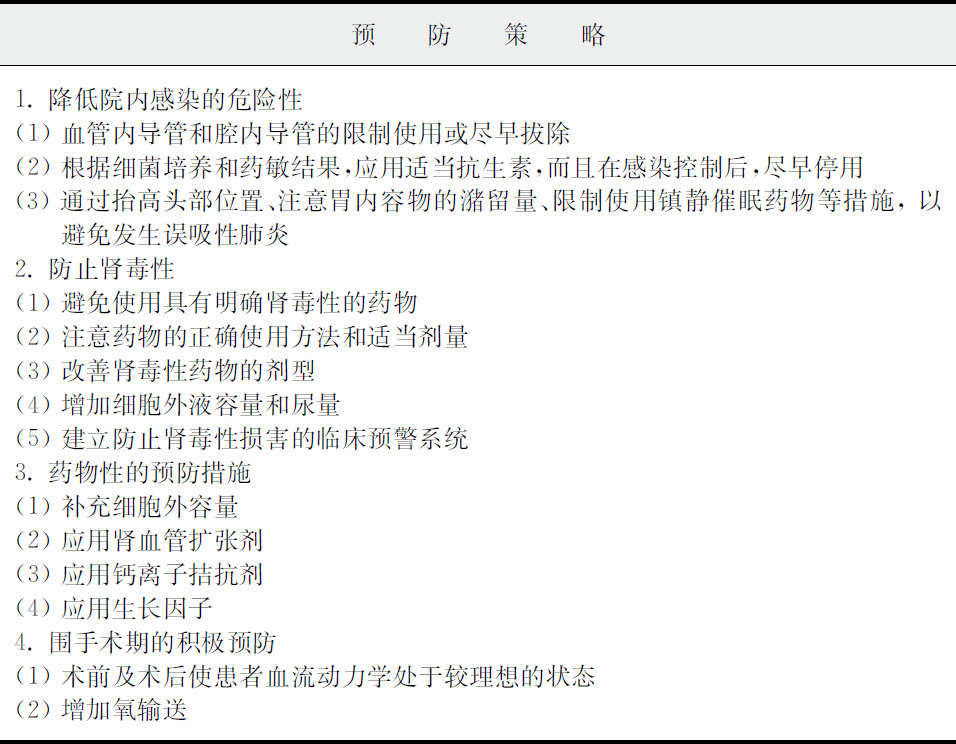
\includegraphics{./images/Image00092.jpg}
\end{table}

(1)术前及术后使患者血流动力学处于理想状态 围手术期肾脏灌注减少是导致术后发生急性肾衰竭的重要原因,防止围手术期肾脏灌注降低,对预防肾衰具有重要意义。由于肾脏的灌注与全身血流动力学状态直接相关,围手术期使患者血流动力学处于理想状态,就有可能防止肾脏低灌注引起的缺血。若在患者实施大血管手术前,先放置肺动脉漂浮导管,监测患者的血流动力学参数,通过补充液体、血浆和全血,使患者处于较理想的血流动力学状态,手术后,同样根据监测结果,指导循环容量的管理,则术后急性肾衰竭患病率和病死率均明显降低。说明围手术期使患者血流动力学处于理想状态,有可能避免肾脏低灌注和缺血,达到防止急性肾衰竭发生的目的。

(2)增加氧输送 氧输送主要由心脏泵功能(心输出量)、动脉血氧饱和度和血红蛋白浓度3个因素决定,是了解和改善全身组织氧供的重要指标。提高氧输送是重症患者治疗的重要目标。通过增加氧输送,可能达到改善组织灌注,纠正组织缺氧的目的。在急性肾衰竭的防治中,围手术期,特别是手术后,通过提高氧输送,有可能达到避免肾灌注减少和肾脏缺血缺氧,防止急性肾衰竭的目的。目前探讨增加氧输送对急性肾衰竭的预防作用的临床研究结果并不一致。因此,增加氧输送对急性肾衰竭的预防作用仍需进一步研究探索。

\subsubsection{利尿剂与甘露醇在急性肾衰竭防治中有何地位?}

呋塞米是一种袢利尿剂,并具有轻度血管扩张作用,是急性肾衰竭治疗中最常用的利尿剂。

近年来认为,呋塞米在急性肾衰竭治疗中主要具有以下作用:①降低髓袢升支粗段的代谢,使之氧耗降低,避免上皮细胞损伤加重;②冲刷肾小管,清除管型和结晶等肾小管腔内阻塞物,保持肾小管通畅;③降低肾小管中血红蛋白、肌红蛋白的浓度,防止蛋白阻塞肾小管;④促进少尿型肾衰转变为多尿型肾衰。当然,肾衰由少尿型转变为多尿型后,液体管理和治疗较为容易,但并不改变肾衰的病程。

大剂量应用呋塞米有明显副作用,主要表现为耳毒性,但也有呋塞米加重造影剂相关急性肾衰竭的报道。另外,也有报道无尿患者反复大剂量应用呋塞米,导致容量负荷增加,引起肺水肿。

呋塞米的使用剂量应逐步增加。初始剂量20mg,1小时后无效,可静脉推注呋塞米40mg。1小时后如仍无效,则静脉注射呋塞米200mg,每小时1次,连用3次。尿量仍无明显增加,则可改为呋塞米持续静脉泵入,剂量为1~4mg/分,可持续使用2~3天。

甘露醇不但具有渗透性利尿作用,还具有清除细胞外氧自由基的作用。在肾移植中,甘露醇作为移植肾的保护剂。甘露醇在急性肾衰竭的防治中应用并不广泛。在挤压综合征引起肌红蛋白尿性急性肾衰竭中,早期应用甘露醇对急性肾衰竭具有治疗作用。其他病因引起的急性肾衰竭中,甘露醇无治疗作用。对于造影剂引起的急性肾衰竭,应用甘露醇反而加重急性肾衰竭。因此,甘露醇在急性肾衰竭的救治中不应常规应用。

\subsubsection{肾脏剂量的多巴胺在急性肾衰竭的防治中还有地位吗?}

一般认为,多巴胺具有选择性肾血管扩张和增加尿量的作用,肾脏剂量的多巴胺(小剂量多巴胺)在临床上被广泛用于急性肾衰竭的防治,但多巴胺上述作用缺乏充分的临床和实验研究证据。研究认为1μg/(kg·分)多巴胺具有肾脏血管扩张作用,而常规应用的剂量为3~5μg/(kg·分),主要表现为缩血管作用,并无血管扩张作用。在安慰剂对照的临床试验中,多巴胺并不能降低急性肾衰竭患者的病死率,而且也不能使透析时间缩短。虽然小剂量多巴胺能够增加患者的尿量,但并不增加肌酐清除率。

对于肾前性肾脏功能损害患者,小剂量多巴胺可通过正性肌力作用,增加心脏输出量,使肾脏灌注部分改善。但是,对这类患者应特别注意有效循环血量不足对肾脏灌注的影响,低灌注状态应及时纠正。否则,应用多巴胺早期或许尿量有所增加,但因有效循环血量和肾脏灌注不足,可导致肾脏损害进一步恶化。

临床研究显示对于肾脏功能轻度受损的重症患者(肌酐清除率70~80ml/分),多巴酚丁胺并不增加患者尿量,但明显增加肌酐清除率,而多巴胺增加尿量,并不增加肌酐清除率,提示多巴酚丁胺能够改善肾脏灌注,而多巴胺仅具有利尿作用。

多巴胺和多巴酚丁胺具有正性肌力作用,通过增加感染性休克和心衰患者的心输出量,改善器官组织灌注,其中肾脏的灌注也可部分改善。但是需注意以下问题:

(1)正性肌力药物结合液体复苏,将氧输送提高到超常水平(supernormal),并不能改善全身性感染及多器官功能障碍综合征患者的预后,提示多巴胺与多巴酚丁胺提高心输出量并不一定能够改善急性肾衰竭患者的预后。

(2)多巴胺的剂量过高将会导致肾脏血管痉挛,使肾脏灌注减少,进一步加重肾缺血和肾损伤。

总之,肾脏剂量的多巴胺并不能改善肾脏灌注。多数学者对多巴胺的肾脏保护作用持怀疑或否定观点。因此,在急性肾衰竭的防治中,肾脏剂量的多巴胺不应常规使用。

\subsubsection{心房利钠肽在急性肾衰竭治疗中可否改善预后?}

心房利钠肽(atrial natriure
ticpeptide,ANP)是近年来治疗急性肾衰竭有一定疗效的药物,主要作用包括:①扩张入球小动脉、收缩出球小动脉,使肾小球滤过率增加;②抑制肾小管对钠的重吸收,总的效应表现为尿量增加。

在动物实验中,ANP能够明显改善缺血性和肾毒性因素引起的急性肾衰竭,甚至在肾脏缺血和肾毒性损害2天内用药,也能改善急性肾衰竭。临床研究初步显示ANP对急性肾衰竭有明显疗效。包括53例急性肾衰竭患者的一个开放性研究显示,应用ANP后,患者肾小球滤过率提高1倍,而需要透析治疗的患者减少了50%。一项多中心随机对照双盲临床试验纳入504例急性肾衰竭的重症患者,结果显示ANP对21天的患者生存率、病死率和血浆肌酐水平无明显影响,ANP治疗组患者21天生存率为43%,对照组为45%。但对其中120例少尿型急性肾衰竭患者进行亚组分析发现,ANP治疗组(60例)患者21天生存率为27%,而对照组(60例)为8%(\emph{P}
=0.008)。可见,ANP能够明显降低少尿型急性肾衰竭患者病死率。另外,有报道认为ANP能够将少尿型急性肾衰竭转变为非少尿型急性肾衰竭,ANP能够减轻肾脏的缺血再灌注损伤
\protect\hyperlink{text00017.htmlux5cux23ch8-16}{\textsuperscript{{[}8{]}}}
,这可能是ANP改善急性肾衰竭患者预后的原因。

总之,ANP可能是能够改善急性肾衰竭预后,并能将少尿型肾衰转变为多尿型肾衰的有效药物之一,值得临床医师重视。ANP具体使用方法是0.2μg/(kg·分)持续静脉泵入,至少连续使用24小时,并根据疗效进行调整。

\subsubsection{胰岛素样生长因子-1是否可用于急性肾衰竭的治疗?}

胰岛素样生长因子(Insulin-like Growth
Factor,IGF)-1也是近年来治疗急性肾衰竭的试验性药物之一。IGF-1在发育的肾脏中具有极高的浓度,其主要作用是刺激细胞增殖和分化。理论上,IGF-1能够促进急性肾衰竭后的损伤细胞功能修复。

在急性肾脏损害的动物模型中,肾脏损伤后24小时给予IGF-1,动物的肾脏损害明显改善。在狗肾移植模型中,IGF-1能够明显防止肾移植后的肾脏损害。最近的研究发现,大鼠动物模型中刺激IGF-1生成,亦可减少肾脏缺血再灌注损伤
\protect\hyperlink{text00017.htmlux5cux23ch9-16}{\textsuperscript{{[}9{]}}}
。提示IGF-1可能能够改善急性肾衰竭患者的预后。但进一步的临床研究并未发现对手术、创伤、低血压、全身性感染等原因导致的急性肾衰竭患者的肾功能、需要透析的比例以及病死率有明显改善作用。目前IGF-1在急性肾衰竭的治疗仍未进入临床,仍需进一步的研究探讨其机制,评价临床疗效。

\subsubsection{发生急性肾衰竭的重症患者代谢有何异常?}

近年来,通过临床和实验研究,人们对重症患者的能量代谢和蛋白质代谢有了较为深入的认识。急性肾衰竭合并多器官功能障碍综合征的患者不但具有一般重症患者的应激代谢反应,还具有其特殊的改变,例如,液体过负荷、肺水肿、代谢性酸中毒、电解质紊乱等。急性肾衰竭的代谢改变主要表现为以下几方面:

(1)内分泌状态的改变 急性应激状态下的内分泌改变主要表现为胰岛素释放增加,同时胰高血糖素、儿茶酚胺、皮质醇等胰岛素拮抗激素释放明显增加,结果导致以血糖增高为主要表现的“胰岛素抵抗状态”,这是急性应激患者的主要代谢改变。急性应激状态下,还常常出现低T3综合征和睾酮水平降低,但胰岛素样生长因子(IGF)常常升高。急性肾衰竭引起的机体应激状态亦可引起上述改变,但急性肾衰竭本身对大多数激素的改变无明显影响。

(2)能量代谢 应激使重症患者的能量代谢明显增加,常常成为“高代谢状态”,但这种“高代谢状态”常常被过高的估计。近年来,通过代谢车在床边常规开展能量代谢测定以来,发现处于应激状态的重症患者的能量消耗,仅比预计的静息能量消耗高20%~30%。

单纯急性肾衰竭患者的能量消耗与正常健康人类似。但对于合并多器官功能障碍综合征的患者或处于应激状态的患者,其能量消耗较预计的静息能量消耗高15%~20%。另外,间歇性血液透析可使代谢率增加15%~30%。

当然,对于严重程度类似的重症患者,合并急性肾衰竭者的能量消耗要略低于非急性肾衰竭患者,其原因主要与急性肾衰竭导致肾脏的能量消耗减少有关(正常肾脏占体重的0.5%,占全身能耗的10%)。

(3)糖代谢 高血糖是最常见的代谢改变,是应激导致胰岛素抵抗的后果。从另一角度来看,血糖增加实际上是机体代偿机制的一部分,保证依赖于血糖浓度的组织代谢需要,如巨噬细胞、内皮细胞、免疫和炎症细胞等。

生理条件下,血糖升高导致胰岛素释放增加,使骨骼肌和脂肪组织对糖的摄取和利用增加。但在胰岛素抵抗状态下,骨骼肌和脂肪组织无法利用糖,而且还需分解氨基酸合成糖。

急性肾衰竭患者糖的氧化利用能力明显降低,糖代谢仅占全身代谢需要的23%,而正常健康人可达39%,慢性肾衰患者也可达到36%。

(4)脂肪代谢 应激及急性肾衰竭状态下,患者三酰甘油及含三酰甘油的脂蛋白的血浆浓度升高,而胆固醇,尤其高密度脂蛋白胆固醇浓度正常或降低。血浆三酰甘油浓度增加与极低密度脂蛋白浓度增加有关,主要与肝脏合成增加及外周脂蛋白脂酶和肝三酰甘油酶的活性降低(约50%)导致脂肪分解与清除率下降有关,即患者对脂肪的廓清能力降低。

尽管脂蛋白脂酶活性降低,但急性肾衰竭患者对外源性脂肪能够很好地代谢利用,加上脂肪具有较低呼吸商,因此,脂肪依然是急性肾衰竭患者的主要能量来源。

(5)蛋白代谢 应激状态及急性肾衰竭时,蛋白代谢受到很大影响。一方面,蛋白质分解代谢明显增强而合成下降;另一方面,蛋白质的代谢转换明显增加,主要表现为蛋白在器官之间转换和器官内的不同蛋白的转换,如骨骼肌蛋白分解增加,肝脏利用氨基酸合成炎症蛋白。氨基酸动力学研究也表明,骨骼肌内支链氨基酸分解增强,亦有研究认为,代谢性酸中毒可诱导肌肉蛋白溶解酶的基因转录(器官内不同蛋白的转换)。另外,代谢性酸中毒及透析治疗本身均可加剧净蛋白分解,最终导致氮丢失增加和负氮平衡。

导致急性肾衰竭的蛋白高分解状态的原因主要包括:①应激导致的激素状态改变,特别是胰岛素抵抗状态;②酸中毒激活蛋白代谢酶。

(6)微量元素和维生素的代谢 由于肾功能障碍,使机体对水分、尿素氮、肌酐及钾、镁、磷等排泄困难而造成水中毒、氮质潴留,高钾、高镁、高磷血症及代谢性酸中毒,机体内环境紊乱。

间歇性或持续性肾脏替代治疗可导致机体的许多营养成分、微量元素和维生素的丢失。硒和维生素E等抗氧化剂水平的降低,使机体处于低抗氧化状态。肾脏羟化酶活性降低,导致维生素D\textsubscript{3}
浓度降低。

\subsubsection{肾脏替代治疗对急性肾衰竭患者代谢有影响吗?}

(1)透析器/血滤器滤过膜对代谢的影响 血液透析器/血滤器滤过膜的生物相容性对机体的影响已受到广泛重视。对于生物相容性差的滤过膜,当血液通过滤器时,不但可激活补体,还可激活粒细胞和血小板,合成和释放细胞因子、蛋白酶等炎症性介质,可使急性肾衰竭的高分解状态进一步恶化。因此,选用生物相容性较好的滤过膜,实施肾脏替代治疗,具有明显的临床价值。

(2)肾脏替代治疗对营养物质的清除 实施肾脏替代治疗时,滤器不但清除尿酸、肌酐等代谢产物,同时也能清除葡萄糖、氨基酸等营养物质,因此,急性肾衰竭患者实施肾脏替代治疗时,应考虑到营养物质的清除问题。营养物质的浓度越高,被清除的量可能就越多。当然,营养物质的清除量不仅与血浆中营养物质的浓度有关,还与滤器的通透性有关。血液透析时,透析器孔径较小,主要通过弥散机制,清除小分子物质;相反,血液滤过或血液滤过透析时,血滤器孔径较大,主要通过对流机制,可清除较大分子量的溶质。因此,需根据肾脏替代治疗手段的不同,分析对营养物质的清除作用。

①对葡萄糖的清除 葡萄糖的分子量较小,可自由通过透析器膜和血滤器膜,因此,血液透析和血液滤过时,葡萄糖的丢失是类似的,为25~50g/天。但是血液透析滤过时,葡萄糖的丢失量可能更多,需予补充。

②对脂肪的清除 由于脂肪在循环中仅以脂蛋白的形式存在,或以与清蛋白结合形式(脂肪酸)存在,脂蛋白颗粒或清蛋白的分子量较大,均无法通过透析器或血滤器膜,因此,肾脏替代治疗时,不考虑脂肪的丢失。

③对氨基酸的清除 氨基酸的分子量较小,血液透析和血液滤过均能清除氨基酸。当使用高流量血液滤过时,氨基酸的丢失尤为显著。对于血滤期间接受静脉营养的患者,静脉营养中大约10%的氨基酸可能经血液滤过丢失。

\subsubsection{急性肾衰竭患者实施营养代谢支持治疗应如何选择营养途径?}

肠道功能基本正常的急性肾衰竭患者,应尽早开始胃肠营养支持,而对于无法利用肠道的患者,应在休克纠正后,立即给予肠外营养支持。

肠内营养支持应使用要素营养液,如爱伦多、能全力、安素等,能量密度为4.184kJ/ml。对于重症患者,可肠道内补充特殊的氨基酸-谷氨酰胺,以促进和改善肠道黏膜绒毛的功能。

对于肠道功能障碍的患者,可采用肠外营养,而对于肠道功能部分受限的患者,可采取肠外营养为主,辅以少量的肠内营养。即使是很少量的肠内营养液,也有助于刺激肠道蠕动,增加肠黏膜血流,改善肠内菌群和黏膜绒毛的功能。

\subsubsection{急性肾衰竭患者实施营养代谢支持治疗的注意事项}

(1)营养液的热量 不同疾病状态的能量消耗量不同,间接测能仪可使能量供给达到较理想水平及实现个体化,一般可在104.6~125.5kJ/(kg·天),但有学者推荐此类患者能量供给在75%静息能量消耗量即可。亦有认为,对透析患者可按125.5~146.4kJ/(kg·天)补充能量。

(2)非蛋白热量 糖、脂双能源可提供非蛋白质热量。临床研究显示,肾功能减退时,机体对外源性脂肪的清除率并未降低,表明对其有较好的耐受力。中长链脂肪乳剂血浆清除快,对糖代谢干扰小,但在其他方面并未显示出更大的优势。此外,血滤或透析同时输注脂肪乳剂,对于滤膜及透析效果并无影响。

肾移植术后患者,由于创伤与大剂量糖皮质激素应用,使葡萄糖耐量下降,血糖升高,甚至出现继发性糖尿病,故应适当限制碳水化合物摄入量。此外,糖皮质激素与环孢素A的作用可使血脂、尤其胆固醇升高。输注ω-3聚不饱和脂肪酸有降低炎症反应、提高移植物存活率作用。

由于肾衰竭时合并水潴留,须限制液体入量,而20%~30%的脂肪乳剂具有小体积提供高能量的优点,尤其是对于非透析的不能耐受较大容量肠外营养液的急性肾衰竭患者,可提高其能量的补充量。脂肪乳剂的热量补充量可达非蛋白热量补充量的40%~50%。

鉴于肾衰时脂肪清除能力下降,在输注脂肪乳剂时应常规进行血脂代谢方面的监测。

(3)氮的供给 在肾衰竭及应激状态下,机体对蛋白质的需要量也是增加的,但由于肾脏排泄障碍限制了蛋白的补充。目前认为,增加氮源的补充量有助于减少体内蛋白质分解及改善肾功能,特别是对于接受血透与血滤的患者蛋白质摄入>1.2g/(kg·天)才可达到氮平衡状态,但具体应根据代谢情况而定。对于未进行透析或血滤的患者应限制蛋白的入量,以免加重氮质血症。

在氮源的选择上,普遍认为宜以补充必需氨基酸为主以及酮类似物等。因为内源性的氮可由酮类似物经转氨作用合成非必需氨基酸而减少体内氮的积蓄。近年来亦有研究认为,输注氨基酸液中必需氨基酸与非必需氨基酸的组分对于肾衰竭的预后并无明显影响。

此外,氨基酸、葡萄糖、维生素与微量元素均可通过透析膜而部分滤出。持续血液滤过时氨基酸丢失明显,无糖透析时有少量葡萄糖丢失,而使用含糖透析液时,有35%~40%的葡萄糖被吸收入体内。脂肪与整蛋白不被滤出,维生素与微量元素的丢失量尚不清楚。所以,应根据透析的具体情况,确定提供的营养素种类及用量。

(4)电解质、微量元素和维生素的补充 应注意在补充能量及胰岛素、纠正酸中毒后,可使钠、钾、镁、磷向细胞内转运而使血浆浓度降低。肾衰竭使调节钙磷代谢的维生素D在肾脏的活化过程受影响,从而影响体内的钙磷代谢,引起骨钙丢失,故应注意钙与维生素D的补充。尤其肾移植术后,糖皮质激素的应用使钙的吸收减少、排出增加,有人认为此类患者每日钙的入量应达800~1200mg。因此,急性肾衰竭患者营养支持中,水、电解质与酸碱平衡的监测是非常重要的。

(5)营养液的容量 补充高浓度的葡萄糖液、氨基酸液与脂肪乳剂,从而减少营养液的总量,以免加重水中毒。

\subsubsection{早期请肾脏科会诊在重症病人急性肾衰竭治疗中有何作用?}

临床流行病学调查显示,肾脏科医师的早期会诊和协助处理,能够明显改善急性肾衰竭患者的预后。最近的研究亦证实,重症医学科急性肾衰竭患者中,高达62.3%的患者肾脏科会诊被延迟或超过48小时,而延迟会诊导致患者的重症医学科病死率明显增高(未延迟会诊组65.4%,延迟会诊组88.2%,P<0.001)
\protect\hyperlink{text00017.htmlux5cux23ch10-16}{\textsuperscript{{[}10{]}}}
。可见,早期邀请肾脏科会诊有助于改善急性肾衰竭患者的预后。

肾脏科会诊的延迟往往与临床医师对急性肾衰竭的认识不足有关。当患者血清肌酐浓度未达到4.5mg/dl或尿量高于400ml时,往往会认为患者肾功能基本正常。较低的血肌酐浓度可能与容量负荷过高引起血浆肌酐稀释及严重营养不良引起肌酐生成减少有关。但这一问题在重症医学科可获得较好的解决。重症医学科医师往往将急性肾衰竭看作是多器官功能障碍综合征的一部分,根据多器官功能障碍综合征的诊断标准,血清肌酐浓度高于2mg/dl就被认为发生肾衰,就会引起重症医学科医师的高度重视,而给予积极处理。

\subsubsection{急性肾衰竭进入多尿期治疗上应注意哪些问题?}

(1)早期 治疗原则为防止补液过多,注意适当补充电解质。

虽然尿量逐渐增多,但患者体内仍处于水中毒的高峰。大量排尿,水分来自于过剩的细胞外液。如果大量补液,势必造成循环负担过重,引起心功能不全、肺水肿,甚至脑水肿。必须防止补液过快、过多,更不可尿多少,补多少。原则上,补液按少尿期处理。当尿量>2000ml/d时,补液量=尿量的1/3~1/2+显性丢失。

如尿量增加不明显,不要立即停止使用多巴胺、呋塞米等药物。

多尿早期血尿素氮仍进行性升高,酸中毒也继续加重,并持续3~4天,应补充足够热量,减少蛋白摄入,给予蛋白合成激素,尽量缩短多尿早期的持续时间,使血尿素氮尽快下降。

由于氮质血症加重,仍可并发严重感染、消化道出血等并发症。如果发生消化道出血,应补充新鲜血,使血细胞比容达到25%左右、血红蛋白>60g/L。

由于大量利尿,应严密监测血电解质的变化,注意适当补充电解质。

(2)中期 治疗原则为适当补液,防止水电解质大量丢失。

此期尿量明显增加,可达4000~5000ml/天以上,甚至>10000ml。补液量应根据监测指标,大约为尿量的2/3。以后随尿量减少,逐渐使入量等于出量。

电解质补充非常重要。主要根据临床生化监测结果补充,临床生化监测有时需要4~6小时进行1次。原则上每1000ml尿量,可补充钾2~3g、补钠3~5g,并同时注意补充钙、镁、维生素等。

随着氮质血症的减轻,临床症状逐渐好转,消化道功能开始恢复,加之尿量增多,应尽早开始口服补充水电解质及热量,逐渐减少肠外营养。但仍需供给足够热量,以利于尿素氮下降,防止感染。

(3)后期 治疗原则为保持水平衡。

随着饮食恢复,应增加饮水,适当控制静脉入量。减少肠外营养,增加胃肠的热量摄入。

恢复期无需特殊治疗,应避免使用肾毒性药物。如必须使用,应根据血浆肌酐清除率适当调整药物使用剂量及给药时间。每1~2个月复查肾功能1次,持续1年以上。

\begin{center}\rule{0.5\linewidth}{\linethickness}\end{center}

参考文献

\protect\hyperlink{text00017.htmlux5cux23ch1-16-back}{{[}1{]}} .Bellomo
R,Ronco C,Kellum JA,et al.The ADQI workgroup:Acute renal failure
--- definition,outcome measures,animal models,fluid therapy and
information technology needs:the Second International Consensus
Conference of the Acute Dialysis Quality Initiative(ADQI).Group.Crit
Care.2004,8:R204-R212.

\protect\hyperlink{text00017.htmlux5cux23ch2-16-back}{{[}2{]}} .Bagshaw
SM,George C,Bellomo R.A comparison of the RIFLE and AKIN criteria for
acute kidney injury in criticallyill patients.Nephrol Dial
Transplant,2008,23(5):1569-1574.

\protect\hyperlink{text00017.htmlux5cux23ch3-16-back}{{[}3{]}} .Bagshaw
SM,George C,Bellomo R;ANZICS Database Management Committee.Early
acute kidney injury and sepsis:a multicentre evaluation.Crit
Care.2008,12(2):R47.

\protect\hyperlink{text00017.htmlux5cux23ch4-16-back}{{[}4{]}} .Lerolle
N,Nochy D,Guerot E,et al.Histopathology of septic shock induced
acute kidney injury:Apoptosis and leukocytic infiltration.Intensive
Care Med.2010,36:471.

\protect\hyperlink{text00017.htmlux5cux23ch5-16-back}{{[}5{]}} .Rivers
E,Nguyen B,Havstad S,et al.Early-directed therapy in the treatment
of severe sepsis and septic shock.N Engl J Med,2001,345:1368-1377.

\protect\hyperlink{text00017.htmlux5cux23ch6-16-back}{{[}6{]}} .Liu
C;Bayer A;Cosgrove SE,et al.Clinical practice guidelines by the
infectious diseases society of America for the treatment of
methicillin-resistant Staphylococcus aureus infections in adultsand
children.Clin Infect Dis.2011,52(3):e18-55.

\protect\hyperlink{text00017.htmlux5cux23ch7-16-back}{{[}7{]}} .Bosso
JA,Nappi J,Rudisill C,et al.Relationship between Vancomycin Trough
Concentrations and Nephrotoxicity:a Prospective Multicenter Trial
Antimicrob.Agents Chemother.2011,55(12):5475.

\protect\hyperlink{text00017.htmlux5cux23ch8-16-back}{{[}8{]}} .Koga
H,Hagiwara S,Kusaka J,et al. Human Atrial Natriuretic Peptide
Attenuates Renal Ischemia-Reperfusion Injury.J Surg Res.2010.

\protect\hyperlink{text00017.htmlux5cux23ch9-16-back}{{[}9{]}} .Harada
N,Zhao J,Kurihara H,Nakagata N,Okajima K.Stimulation of Fc gamma RI
on primary sensory neurons increases insulin-likegrowth factor-I
production,there by reducing reperfusion-induced renal injury in
mice.J Immunol.2010.185(2):1303-1310.

\protect\hyperlink{text00017.htmlux5cux23ch10-16-back}{{[}10{]}} .Ponce
D,Zorzenon CP,dos SNY,Balbi AL.Early nephrology consultation can
have an impact on outcome of acute kidneyinjury patients.Nephrol Dial
Transplant.2011.26(10):3202-3206.

\protect\hypertarget{text00018.html}{}{}

